%!TEX root = ../BoYu-Dissertation.tex
\graphicspath{{Figures/}}

\chapter{Promoting Event-Driven Awareness} % (fold)
\label{cha:promoting_event_driven_awareness}
In this chapter, we discuss our approach to promoting the event-driven awareness. More specifically, we address three major design components: (1) local space-based event notification mechanism, (2) a visualization framework for supporting event interpretation, and (3) interactive tools to support event propagation. The three components contribute to the different stages of the awareness development process. The event notification mechanism focuses on supporting the awareness perception by filtering out the events and controlling the notification styles. The visualization framework for event interpretation aims to support the development of higher level awareness, including both comprehension and projection. Supporting event propagation relates to the social processes to establish compatible awareness across multiple actors.

Each component is designed to follow the two design principles outlined in Chapter \ref{cha:our_approach_overview}:
\begin{enumerate}
	\item We emphasize how the computer's knowledge representation of the field of work and events are utilized in each component.
	\item We attempt to strike a balance between the system's computational and reasoning capabilities to reduce human effort and providing interactive support to keep human actors in the loop and retaining control.
\end{enumerate}

\section{Event Notification Mechanism} % (fold)
\label{sec:event_notification_mechanism}
As we discussed in Section \ref{sub:awareness_processes_in_event_based_models}, the event perception is usually supported by event notification mechanisms \cite{McCrickard2003}. In this study, we distinguish \emph{events} from \emph{event notifications} as follow: while an event represents the information about a real-world occurrence or some aspect of actor's interpretations necessary to provide awareness, multiple notifications about that event can be directed to multiple receivers if it is relevant to them. Each event notification includes not only the content of the corresponding event, but also the actor who will be informed, as well as the notification style, i.e. the appropriate way to present the notification.

Event notifications are generated through event subscription and filtering mechanism. A subscription describes a set of notifications a user is interested in. The user register the interest in receiving certain kinds of notifications by submitting subscriptions to the computer system. The system filters incoming events based on the subscriptions and delivers those notifications that match one of the user’s subscriptions. 

As we discussed in Section \ref{ssub:support_for_perception}, several ways to specify interests and filter out events have been used in existing awareness systems, which offer different degrees of expressiveness and overhead on the users. Topic-based or type-based mechanisms are rather static and primitive, but can be implemented very efficiently and requires less effort for the user to manage the subscriptions. On the other hand, content-based mechanisms are highly expressive, but requires sophisticated protocols that have higher overhead to manage the subscriptions. This section provides the design of event notification mechanism in our approach. The major difference of our approach from existing studies is that we leverage the system's knowledge about each actor's local scopes to provide a two-tier notification mechanism that can combine the benefits of both topic-based and content-based mechanisms. 

Our design of local scope-based event notification mechanism is based on the assumption that human actors in a collaborative activity are only interested in events that have impact on their individual working context, i.e. defined as their local scopes. Following this, our event notification mechanism is performed in two steps (Figure \ref{fig:event_filtering}):
\begin{enumerate}
  	\item Given an event instance and an actor, the event is first filtered based on whether it is associated with any entity in the actor's local scope of work. 
  	\item If the event passes the first step, i.e. it is within the actor's local scope of work, the local scope-based subscriptions managed by the actor are applied to further filter the event and decide on the notification style for the event.
  	\item If the event does not pass the first step, it is sent to a standard content-based notification module to further decide on its relevance to the actors.
\end{enumerate}  

\begin{figure}[htbp] %  figure placement: here, top, bottom, or page
	\centering
	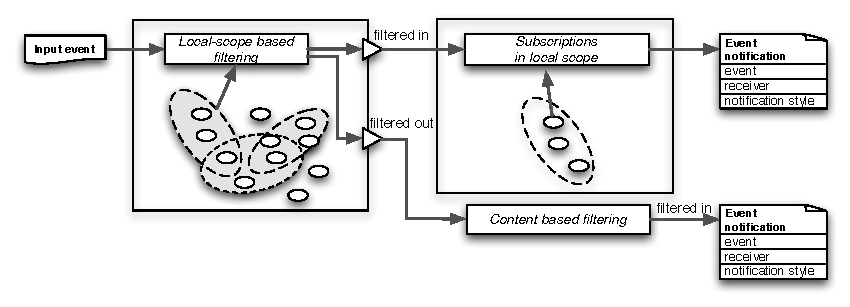
\includegraphics{event_filtering.pdf} 
	\caption{Local scope-based event filtering}
	\label{fig:event_filtering}
\end{figure}

The first step of filtering events based on an actor's local scope is very similar to the topic-based methods, as it introduces a programming abstraction to divide the event space into multiple sub-spaces. Then the filtering process is to determine whether the event falls into any of these sub-spaces. However, the major difference is that, while the concept of topic is usually static, the local scope is a dynamic concept. As we define the local scope as the actions in the field of work that an actor imposes certain level of intention or capability ( Section \ref{sub:local_scopes}), it is likely that it will be modified as the actor works on different tasks or the environment changes. The knowledge updating process as we describe in Section \ref{sec:knowledge_updating_process} allows the system to ensure that its representation of actors' local scopes is always updated to current state. As a result, the events that pass the first step are always relevant to the actor's current working context. 

The second step in our method allows the users to further specify how they want to be notified for these events within their local scopes. Because the events that are passed into this step are limited to those within each actor's corresponding local scope, the total number of events that each actor needs to manage is greatly reduced.

Considering the knowledge updating process mentioned in Section \ref{sec:knowledge_updating_process}, not all the events can be successfully associated with entities in human actors' local scopes by the computer system. The system may not be able to recognize the relevance of some external events during the association and assessment steps at first, but rather depends on the human actors to interpret them and generate internal events that can be recognized later. For these events, we should still allow the users to subscribe to them using the content-based mechanisms. Because the events that need to be managed using the content-based mechanism are only a small subset that cannot be associated with local scopes, the overhead on the users to manage them are minimized.  

In the following of this section, we focus on the local scope-based filtering and subscription mechanism. We first describe the algorithm to perform the local scope-based filtering in the first step, and then discuss the management of subscription within the local scopes. The content-based notification mechanisms have been well discussed in the literature on event-based computing \cite{eugster2003many}, and many existing event infrastructures provide support to it, so we do not provide detail here. Readers can refer to \cite{Mhl2010} for more discussion.

\subsection{Filtering events by local scopes} % (fold)
\label{sub:event_filtering_algorithm}
To filter events based on local scopes, we need to make use of the system generated knowledge attached to each event during the knowledge updating process, i.e. before an event is sent to the notification component, it should have been processed to update the system knowledge following the steps described in Section \ref{sec:knowledge_updating_process}. As a result, every input event in the filtering operation is already transformed into an \emph{event chain} $EC=(e_0, e_1, e_2, ...)$ that includes at least one original event $e_0$, and possibly additional derived and anticipatory events. If any event in the event chain has references to entities in the PlanGraph model, such references should have been established during the knowledge updating process.

Therefore, filtering the event by local scopes is the operation that takes an event chain $EC$ and an actor $ar$, and then finds whether any event instance in the event chain is relevant to the user based on $ar$'s local scope. The operation can be performed in the following steps:

\begin{enumerate}
	\item The local scopes of the actor $ar$ is constructed from the current PlanGraph $PG$, following the algorithm described in Section \ref{sub:representing_local_scopes}.
	\item For each event instance in the event chain $EC$, we first iterate through its attributes to check whether it has references to entities in the PlanGraph model. If none is found, the event instance is skipped.
	\item If the event instance is found to have references to entities in the PlanGraph model, we check whether any entity is inside the local scope of $ar$. If so, we can claim that the event instance passes the filter.
\end{enumerate}

The process can be described as a procedure $FILTER\textrm{-}LS$ as follow.

{\footnotesize
\begin{algorithm}
\begin{algorithmic}[1]
\Procedure{FILTER-LS}{$EC,ar$}
	\State $LS = BUILD-LS(ar, PG)$\Comment{construct the local scope}

	\ForAll{$e$ \textbf{in} $EC$}
   		\ForAll{$attr$ \textbf{in} $e.payload$}
   			\If{$typeOf(attr) == EntityReference$}
   				\ForAll{$entity$ \textbf{in} $LS$}\Comment{each entity is a tuple of $\{ar, act, int\}$}
   					\If{$entity[1] == attr$}\Comment{A match is found}
   						\State \textbf{return} $\{e, ar\}$ 
   					\EndIf
				\EndFor

   			\EndIf
   		\EndFor
	\EndFor
	\State \textbf{return} $null$ 
\EndProcedure
\end{algorithmic}
\end{algorithm}
}
% subsection event_filtering_algorithm (end)
\subsection{Managing subscriptions in local scopes} % (fold)
\label{sub:managing_subscriptions}
Once an event passes the local scope-based filtering, the corresponding actor's subscriptions within the local scope are applied to decide on whether and how the event should be notified. 

Each subscription in the local scopes is defined as the pair of an event pattern and a notification style: $sub=(pat, ns)$, where the event pattern $pat$ is specified by means of one or more user-defined filter expressions. Each filter expression takes the form of a predicate that is evaluated against an event. The event passes the filter if the predicate evaluates to $TRUE$, and fails the filter if the predicate evaluates to $FALSE$. Within an actor's local scope, three kinds of filter expression can be attached, and it is possible to mix these different kinds of expressions in one single event pattern:

\begin{enumerate}
	\item An \emph{event type} filter expression lists one or more event types. The expression evaluates to TRUE if the incoming event is an instance of any of these types.
	\item An \emph{event content} filter expression is evaluated from the values of payload attributes of the event instance. For example, $(attrA == valueX)$ and $(attrB > valueC)$.
	\item A \emph{local scope} filter expression is evaluated based on the different intention and capability levels of entities associated with the event. For example, the user may specify an event pattern to match all the events attached to actions that the user is \emph{intended to} perform and are \emph{workable}.
\end{enumerate}

While the event type and content filters can use the same syntax as existing content-based filter expression languages, but the local scope filter expression is unique in our approach and provides an additional level of expressiveness than merely content-based subscriptions. It allows the human actors to describe event patterns based on the relations between the actor and the entities in the local scope, instead of the attributes of an event directly. It is quite common that the actor wants to treat events related to all the actions he/she has certain level of intention in the same way, but cannot specify what exactly these actions are as their local scopes are changing.

Along with each event pattern, the user needs to select a notification style for it. It has to be considered that there is a multitude of different notification styles with different trade-off between its potential to attract attention and its obtrusiveness \cite{Rauschenbach1996}. Generally, we defined five notification styles. 
\begin{enumerate}
	\item The first style is actually not to present the notification at all. This provides another level of control for the users to filter out some events even when they fall into their local scopes.
	\item The object-coupled notification presents some of the event attributes (e.g., time stamp or type) as graphical attributes of the icon representing the entity which is affected by the event. This provides less obtrusiveness to the user but is not perceivable unless the entity is within the user's viewport.
	\item The standalone event window presents a dedicated window to display all the event notifications. It allows the user to keep track of different incoming events at the same place, but loses the visual connections between the events and their references.
	\item Non-modal global notification presents each incoming event at a dedicated corner for a period of time and then disappears. It is more perceivable to the users, but requires the user to respond in a limited time.
	\item Modal global notification uses a modal dialogue box to present a detailed description of an event, and the user has to take an active action to confirm the reception of the event (e.g. click the `close' button) before going back to previous view. 
\end{enumerate}

To support the management of subscriptions within the local scope, the computer system can provide an interactive subscription tool as presented in Figure (??). As the system maintains the knowledge representation of the field of work and each user's local scope, it is easy to generate a diagrammatic representation of the field of work with the user's local scope of work highlighted. Such a visual interface allows the user to perform several tasks to manage the subscriptions:

\begin{enumerate}
	\item The user can easily recognize what actions the system believes are part of his/her local scope. In case the user believes the system's representation is incorrect or wants to make changes, he/she can directly manipulate the visual representation to add/remove entities from the local scope.
	\item The user can click on each of the nodes in the visualization to review active filters on each node, or create new filters. 
\end{enumerate}

\fxwarning{add the figure of the subscription interface. The discussion is incomplete as well.}

% subsection managing_subscriptions (end)

% section event_notification_mechanism (end)

\section{Supporting Event Interpretation} % (fold)
\label{sec:supporting_event_interpretation}
In our approach, we use the term `event interpretation' to include both the process of \emph{comprehension}, i.e. understanding the meaning of perceived event within the context of a user's current goals and activities, and the process of \emph{projection}, i.e. predicting the future states based on the comprehension. Although these two awareness processes have different characteristics at the conceptual level, they are usually inseparable from the user's perspective. The user can switch back and forth between comprehension and projection upon perceiving an event without realizing the difference between them. Hence, we design for supporting event interpretation as an integrated cognitive process that covers both comprehension and projection.

Generally, we consider the event interpretation process as an analytical reasoning process triggered by perceiving an event notification. It includes three interleaving tasks:
\begin{enumerate}
	\item Understanding the meaning of an event within the context of its origin of occurrence. This includes identifying the objects or relations that are mentioned in the event, and understanding what aspects of the objects or relations are changed. 
	\item Assessing the impact of the event on the user's current work context. This includes identifying which part of the actor's work is impacted by the event and what the consequences are.
	\item Predicting the future states on other part of the actor's work or other actors' work because of the dependencies among activities.
\end{enumerate}

In our approach, this analytical reasoning process can be supported from two aspects:

One one hand, the system can perform the reasoning tasks for the user. Actually, as we can see in Section \ref{sec:knowledge_updating_process}, some of these reasoning tasks have already been performed by the system during the knowledge updating process. During the \emph{association} step, the system attempts to identify the objects or relations that are mentioned in the event. In the \emph{assessment} step, the system evaluates the consequences of the event on all the entities in the field of work. In the \emph{propagation} step, the system also predicts the future states on other activities. Hence, the system can support the user by simply present its reasoning results. In this way, some of the high level cognitive tasks are transformed into low level perceptual tasks for the user.

On the other hand, the system can provide external representations of the contextual information to help the users perform these reasoning tasks. As these reasoning tasks are always performed within certain contexts, such as the context of an event's origin, the user's current work context, or the dependencies among activities, the visualization of the contextual information serves as an important cognitive resource for the users.

From the above discussion, we present an information visualization framework for supporting event interpretation with three different types of visual representations (Figure \ref{fig:event_interpretation}):

\begin{figure}[htbp] %  figure placement: here, top, bottom, or page
	\centering
	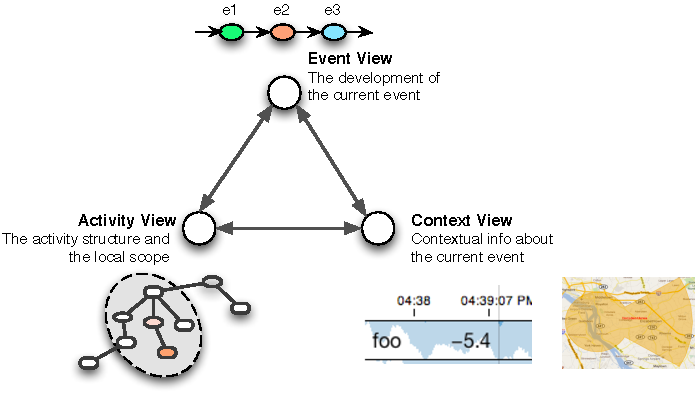
\includegraphics{event_interpretation.pdf} 
	\caption{The visualization framework for event interpretation}
	\label{fig:event_interpretation}
\end{figure}

\begin{enumerate}
	\item Event view: visual representation of the event that needs to be interpreted.
	\item Activity view: visual representation of the field of work and the actor's local scope.
	\item Context view: visual representations of the contextual information that is necessary to interpret the event.
\end{enumerate}

\subsection{Event view} % (fold)
\label{sub:event_view}
The event view is used to present the information about the event that needs to be interpreted. This includes not only the event that is notified to user, but also the whole event chain that the current event is situated in. As we defined in Section \ref{sec:knowledge_updating_process}, an event chain records the development of an event in the knowledge updating process. In the assessment step, the system may generate derived events indicating the system's belief on how the field of work has been changed due to the original event. In the propagation step, the system predicates the future state changes, and add them as anticipatory events into the chain. In this way, the event chain actually represents the results of the system's reasoning on it. 

Therefore, the event view is a diagrammatic representation including an ordered list of nodes (Figure \ref{fig:event_chain}). Each node represents an event in the corresponding event chain. The nodes are arranged in the development order of the events they represent. In a horizontal layout, the node at the most left represents the original event, and then is connected to the set of nodes representing the derived events, followed by the nodes for anticipatory events. The design detail about the event view is summarized as follow:

\begin{figure}[htbp] %  figure placement: here, top, bottom, or page
	\centering
	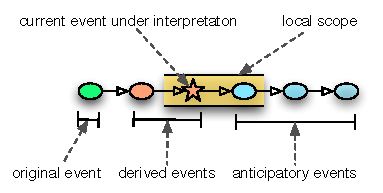
\includegraphics{event_chain.pdf} 
	\caption{Visualizing the event chain in the event view}
	\label{fig:event_chain}
\end{figure}

\begin{enumerate}
	\item The node representing the current event that is notified to the user for interpretation is marked with a star, so that the user can know where the current event under interpretation is situated in the event chain.
	\item The nodes representing events inside the user's local scope are shadowed so that the user can clearly see when the development of the event enters its work context.
	\item The different types of events, i.e. original event, derived events, and anticipatory events, are distinguished by different colors.
	\item We use different opacity levels to indicate the system's confidence level on the anticipatory events.
	\item Clicking on the node will show the detail information about the represented event. If the event is associated with the objects represented in the context view or the entities represented in the activity view, they will be highlighted.
\end{enumerate}
 
 The event view plays two important functions during the event interpretation process. First, the event chain provides an overview of the system's reasoning process of an event, which allows the users to understand where an event comes from, and the possible consequences it leads to based on the system's reasoning. Second, it serves as a navigation interface that allows the user to click on nodes to check details on each step of the reasoning. In next section, we will introduce a revised version of the event view that can play the third function in event propagation to present the development of an event across multiple actors.
% subsection event_view (end)

\subsection{Activity view} % (fold)
\label{sub:activity_view}
The activity view provides an overview of the field of work and the user's local scope. Such a representation provides the information about the goals, actions, resources, and actors that are participated in the collaborative activity and the relations between these different entities. As argued by Carroll et al. \cite{carroll2003a}, such an external representation of the overall situation is very important for awareness development when group work is distributed and many dependencies exist in the collaborative activity. Within the context of event interpretation, we believe the activity view can provide several kinds of support to the user:

\begin{enumerate}
	\item It provides the activity-related frame of reference to understand an event and the system's reasoning on it. The activity view is linked to the nodes in the event view. Whenever the user looks at an event node that is associated with an entity in the field of work, the corresponding object in the activity view is highlighted. Thus, the user can perceive which part of the activity is impacted by the event.
	\item It provides the contextual information from the perspective of the collaborative activity that is necessary for the user to perform reasoning. The activity view allows the user to navigate through the different entities in the field of work, check the detail on each entity, and recognize the different relations between them, which is very important for the user to evaluate and predict the impacts of an event.
	\item It shows the boundary between the entities inside and outside the user's local scope, so that the user always know what part of the field of work he/she needs to focus on.
\end{enumerate}

The activity view consists of a diagrammatic representation of the entities and relations in the field of work, and an interaction interface to navigate through the view. The generation of the activity view is straightforward in our approach. As we maintain the knowledge representation of the whole field of work in the PlanGraph model, it can be easily externalized into a graph visualization with the entities as nodes, and the relations as links. The interaction interface allows the user to perform actions such as zoom in/out, move the viewport, check details, and dynamic queries.

A key issue in designing the activity view is the problem of \emph{discernibility} in graph visualization when the number of elements is large \cite{Herman2000}. It is well known that comprehension and detailed analysis of data in graph structures is easier when the size of the displayed graph is small. Displaying an entire large graph may give an indication of the overall structure, but makes it difficult to comprehend the details. 

To address this problem, we treat the entities inside and outside the local scope differently when visualizing them in the activity view (Figure \ref{fig:activity_view}):
\begin{figure}[htbp] %  figure placement: here, top, bottom, or page
	\centering
	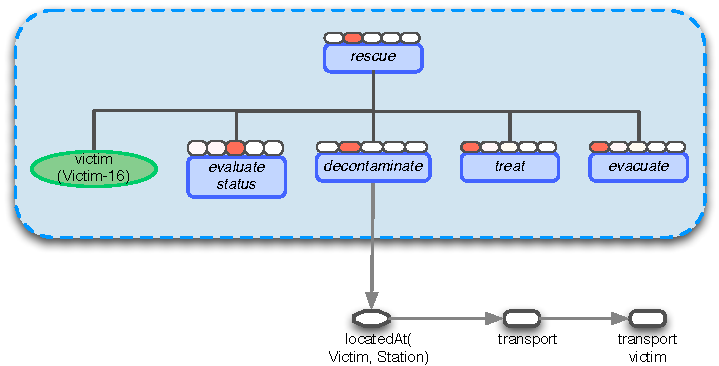
\includegraphics{activity_view.pdf} 
	\caption{Visualizing the field of work in the activity view}
	\label{fig:activity_view}
\end{figure}

\begin{enumerate}
	\item The entities within the local scope are visualized as larger nodes that allows to encode more detailed information, such as the name, type, and execution state. But the entities outside the local scope are visualized as small icons that have less information encoded. 
	\item The different relations between entities with in the local scope are considered and visualized using different types of line styles, but the entities outside the local scope are connected merely based on the dependencies. 
	\item The entities in the local scope are visualized using the hierarchical layout that emphasizes the decomposition relations among actions. The entities outside adopt a more space-efficient graph layout (e.g. force-directed layout \cite{Fruchterman1991}) to show a maximum number of nodes within the limited view port.
\end{enumerate}

The distinction between the entities inside and outside the local scope in the activity view complies with the distributed nature of the field of work. As for each actor, the local scope is where he/she possesses more control and also is the most likely place where the event interpretation will occur. As a result, the user would like to see more details on the entities within the local scope. Meanwhile, the entities outside the local scope are distant from his/her work focus, and all he/she needs to know is how these entities are related to the local scope, with less detailed information about them.
% subsection activity_view (end)

\subsection{Context view} % (fold)
\label{sub:context_view}
The context view is a container for interactive information visualization tools to understand the different contexts of the event, including the the context of an event's origin, the user's current work context, or the dependencies among activities. The contexts emerge from a complex mix of entities in the field of work, including the objects that the user is working on, the collaborating actors, resources, and informational objects that are necessary to understand the situation. In relative simple collaborative environments, such as the collaborative editors, the context can be represented as one single shared workspace. But in complex, real-world collaboration, the contextual information is usually in diverse forms and should be understood from different perspectives. As a result, the context view is usually a set of coordinated and multiple views to represent different perspectives of the context. For example, it may include a cartographic map to display the distribution of actors, a data table to list all the available resource, a time line to show the historical usage of a resource, as well as other diverse visual displays including scatter plots, parallel coordinate plots, histograms etc. The set of views and interactive tools that are needed usually depends on the application domain and each actor's task in the domain.
% subsection context_view (end)
% section supporting_event_interpretation (end)

\section{Mediating Event Propagation} % (fold)
\label{sec:mediating_event_propagation}
Event propagation refers to the social process to establish compatible awareness across multiple actors. As we argue in Section \ref{sec:integrated_conceptual_model_of_awareness}, an essential aspect of the awareness phenomena in distributed, complex collaboration is that the development of awareness should be considered as a social process that can involve a series of interactions among multiple actors. With aspect to the event-driven awareness process, that is to say the awareness process triggered by one event can be developed by multiple actors. The actor who receives the initial event generates his/her own interpretation of the event, and then externalize the interpretation as a new event, which is then received by the second actor. The second actor's interpretation is built on top of the first actor's, and may generate new events that are received by other actors. In this way, as the initial event is propagated to multiple actors, the team awareness is developed.

Unlike the event notification and event interpretation that are operated on each single event, each event propagation process can be considered as a meta-process that consists of multiple processes on multiple events. Figure \ref{fig:event_propagation} shows an example of the event propagation process that involves the computer system and three human actors. In the beginning, an input event $e_0$ is received by the system and the system derives a new event $e_1$ during its knowledge updating process. This derived event $e_1$ indicates a state change of an action that falls into $actor 1$'s local scope, hence it will be notified to $actor 1$ during the notification process. Upon receiving the notification, $actor 1$ performs his/her own interpretation process, and externalize the result of the interpretation as a new event $e_2$. $e_2$ is sent back to the system during the externalization process. After receiving $e_2$, the system starts another round of knowledge updating and notification, and finds that $e_2$ falls into $actor 2$'s local scope. As a result, the system notifies $actor 2$ about $e_2$. The process continues as $actor 2$ further interprets the event and generates new event, which is later notified to $actor 3$.

\begin{figure}[htbp] %  figure placement: here, top, bottom, or page
	\centering
	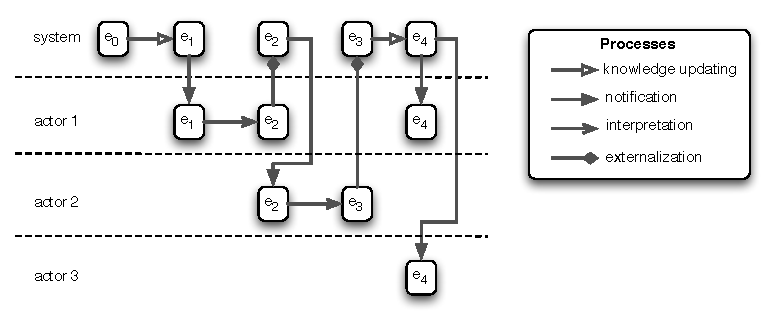
\includegraphics{event_propagation.pdf} 
	\caption{An example of the event propagation process}
	\label{fig:event_propagation}
\end{figure}

From the example, we can clearly see that the event propagation is achieved by the joint effort of the human actors and the computer system. One one hand, it relies on the human actors to interpret the events built on top of other's interpretation, and externalize their own interpretations as new events. On the other hand, the system should be able to disseminate these new events to the actors who are interested in further developing them.

The capability of system to disseminate these derived events to relevant actors can be achieved through the local scope-based event notification mechanism as we described in Section \ref{sec:event_notification_mechanism}. Because the relevance of events to the actors are judged by whether they are associated with the entities in the actors' local scopes, the actors do not need to subscribe to them in advance. As long as the new events generated by other actors fall into my local scope, I will get notified.  

\fxwarning{more discussion on how the propagation works: the basic assumption is the connectivity of local scopes. through shared entity and dependencies.}

Beyond that, the system can mediate the event propagation from the human actor's perspective, i.e. to help the human actors do their jobs in propagating events. The human actors have to be enabled to:

\begin{enumerate}
	\item keep track of the historical development of the event so that they know where an event comes from, how it has been developed, and the actors who have contributed to its development.
	\item easily externalize their interpretation of the event, i.e. how their intentions and beliefs are changed because of the event.
	\item control the visibility of their newly generated events, such as who should be able to receive their interpretation, and to what level of detail.
\end{enumerate}

The following of this section focuses on how these tasks can be achieved by human actors with the computer system's assistance. It requires several enhancements in the knowledge updating process, the event notification mechanism, and the visualization framework for event interpretation, so that the social aspect of the event propagation is explicitly represented and supported.

\subsection{Tracking event propagation} % (fold)
\label{sub:tracking_event_propagation}
In order to keep track of the event propagation, we extend the concept of \emph{event chain} to the concept of \emph{event propagation tree}, and thereafter revise the event view in the visualization framework to represent the event propagation tree. 

In Section \ref{sec:knowledge_updating_process}, we introduce the concept of \emph{event chain} to record the system's development of an event in the knowledge updating process. Now, we extend it to the concept of \emph{event propagation tree} to keep track of the event propagation process from the following two aspects:

\begin{enumerate}
	\item As the event propagation is a meta-process that can involve both the computer system's knowledge updating process and human actors' awareness processes, the events in an \emph{event propagation tree} include not only the events generated in the system's reasoning process, but also those generated by the human actors in the externalization process.
	\item In the event propagation process, it is possible that one event is interpreted by multiple human actors, along with the system's reasoning on it. One event can then be derived into multiple branches, each of which can be further developed into multiple subsidiary branches. As a result, an \emph{event propagation tree} $EPT$ can no longer be represented as a linear sequence of events, but rather a tree structure (Figure \ref{fig:event_propagation_tree}). The root node in the tree structure $e_0$ represents the original event that triggers the propagation, and each node can have multiple branches indicating how the event represented by the node is further developed.
	\begin{figure}[htbp] %  figure placement: here, top, bottom, or page
		\centering
		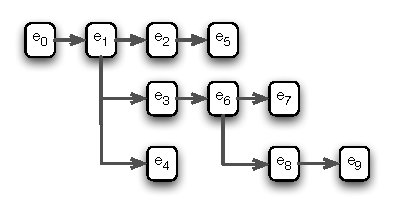
\includegraphics{event_propagation_tree.pdf} 
		\caption{The event propagation tree}
		\label{fig:event_propagation_tree}
	\end{figure}
\end{enumerate}

Similar to the \emph{event chain}, the structure of an \emph{event propagation tree} can be represented in our event representation by adding attributes in the \emph{open content} section of each event (Figure \ref{fig:event_propagation_tree_representation}): 
\begin{enumerate}
 	\item A text string (\emph{label}) indicates the functional role of the event in the event chain, i.e. whether the event is an \emph{original} event, a \emph{derived} event, or an \emph{anticipatory} event.
 	\item An event reference (\emph{parentEvent}) points to the parent event where the current event is derived from. 
 	\item A list of event references (\emph{childrenEvents}) points to all the event that are derived from the current event.
 \end{enumerate} 

In addition, the \emph{event source} attribute in the \emph{header} section indicates the producer of each event, which can be the computer system or one of the human actors.
\begin{figure}[htbp] %  figure placement: here, top, bottom, or page
	\centering
	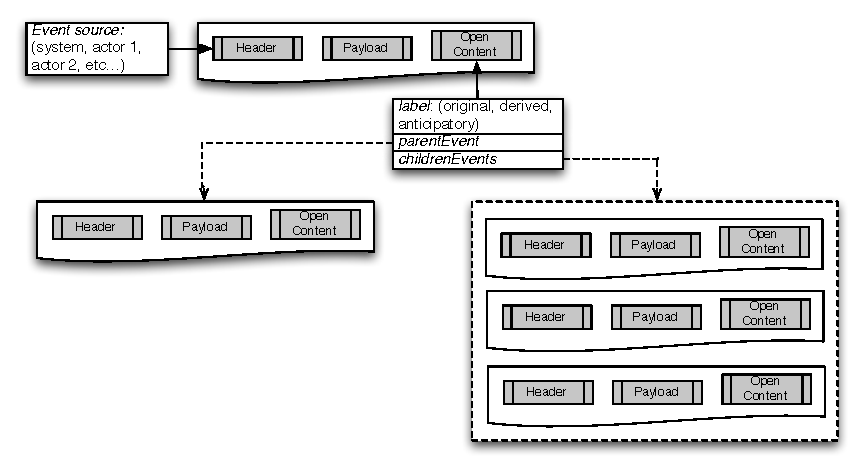
\includegraphics{event_propagation_tree_representation.pdf} 
	\caption{Event structure in an event propagation tree}
	\label{fig:event_propagation_tree_representation}
\end{figure}

By recoding the event propagation tree in the system's knowledge representation, the system can help the human actors to keep track of the event propagation by providing an extended version of the event view in the visualization framework to represent the event propagation tree. Comparing with the original event view, this extended event view provides an overview of the whole event propagation process, not only the results of the system's reasoning, but also how the other actors have contributed to it.

Initially, the extended version of the event view uses a history tree representation \cite{Shrinivasan2008} to visualize the whole structure of an event propagation tree (Figure \ref{fig:extended_event_view}(a)). The event propagation tree is drawn using a right heavy horizontal-vertical tree layout. A horizontal link indicates that the event on the right is derived from the left one. A new branch is created below existing ones in the vertical direction. 

To understand the social context of the event propagation, it is important to see the actors who are participated in the development process and distinguish the events generated by different actors. In order to achieve this, we adopt a complementary layout that divides the visualization space into multiple horizontal rows, and each row only contains the events generated by a particular actor. However, presenting the whole event propagation tree in this layout can cause crossing edges that undermine the discernibility. Hence, we only use this layout to visualize the \emph{active event propagation chain}. We define the \emph{active event propagation chain} as the path from the root node of the event propagation chain to the node that represents the current event under interpretation. Figure \ref{fig:extended_event_view}(b) shows an example of visualizing the active event propagation chain in this layout. The user can toggle between these two representations via the interface. 

\begin{figure}[htbp] %  figure placement: here, top, bottom, or page
	\centering
	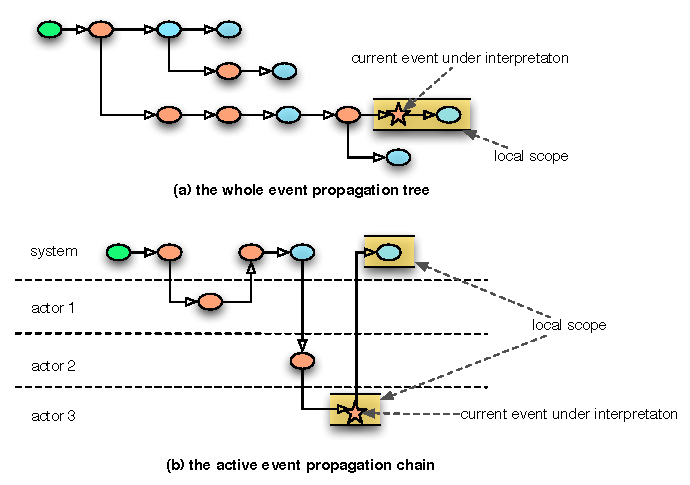
\includegraphics{extended_event_view.pdf} 
	\caption{Visualizing the event propagation tree in the event view}
	\label{fig:extended_event_view}
\end{figure}
% subsection tracking_event_propagation (end)

\subsection{Supporting externalization} % (fold)
\label{sub:supporting_externalization}
Externalization is the process that the human actors express the results of their interpretation of an event as internal events and send them to the computer system for further processing. An important characteristics of these internal events is that they are always associated with certain entities or relations in the PlanGraph model, as they reflect the changes of human actors' internal mental states in the field of work. As a result, we support the externalization by allowing the human actors to directly manipulate the nodes in the activity view where they can create internal events expressing their intentions or beliefs on corresponding entities in the field of work.

Whenever the human actor selects a node in the activity view, the option to create new events will become available in the interface (e.g. in the context menu or toolbar). The types of events that a human actor can generate on each node depends on the type of the corresponding entity in the PlanGraph, i.e. whether it is an action, a parameter, or a condition, and whether it is inside the human actor's local scope or not. 

For an action node inside the local scope, the human actor can generate the following types of events:

\begin{enumerate}
	\item \emph{Intention events}. The human actor can create intention events to indicate the change of intention type (i.e. $Pot.Int$, $Int.Th$, or $Int.To$) toward the selected action.
	\item \emph{Belief events about the capability}. The human actor can create belief events to indicate the change of his/her capability (i.e. $Knows$, $Able$, or $Workable$) of performing the selected action.
	\item \emph{Belief events about the execution states}. The human actor can also create belief events to indicate his/her belief in the execution state change of the selected action.
	\item \emph{Belief events about the plan}. The human actor can also create belief events to modify the current plan of an action. On one hand, the human actor can indicate that he/she believes that the selected action is not part of the plan to performing the parent action, i.e. the current node should be deleted from the PlanGraph. On the other hand, the human actor can elaborate the selected action by adding a new parameter, condition, or subsidiary action to it.
\end{enumerate}

For the parameter nodes inside the local scope, the human actor can also generate belief events about the execution states or contribute to the plan in the similar way as action nodes. However, an additional type of event is available for the parameter nodes, that is the human actor can express the assignment of a particular resource to the selected parameter as a belief event. To allow the human actor to externalize such type of events, a data table containing the list of available resources for the parameter will be displayed so that the human actor can select from the list.

For the condition nodes inside the local scope, belief events about the execution states or plan are also available. Besides, the human actor can create belief events to indicate the modification of the variables in a condition expression. For example, for a condition node representing the temporal constraint on a delivery action, i.e. the delivery must be completed before a given time, the user can select the node and create new event to modify the delivery time. 

For the action nodes outside the local scope, only the intention events and belief events about the capability are available, as the human actor does not have control on the actions that are out of his/her local scope. However, the intention events and belief events about the capability provide a way for the human actor to expand his/her local scope to the outside nodes.

Table \ref{tab:event_types_for_externalization} shows a summary of the different types of events that can be externalized on each type of node in the activity view. 


\begin{table}[htbp]
\centering
\footnotesize
\begin{tabular}{>{\raggedright}p{1.5in}>{\raggedright}p{2.6in}}
\toprule 
\textbf{Node type} & \textbf{Available event types for externalization}\tabularnewline
\midrule 
Action node inside the local scope & 1. Intention events

2. Belief events about the capability

3. Belief events about the execution states

4. Belief events about the plan\tabularnewline
\midrule 
Prameter node inside the local scope & 1. Belief events about the execution states

2. Belief events about the plan

3. Belief events about value assignment\tabularnewline
\midrule 
Condition node inside the local scope & 1. Belief events about the execution states

2. Belief events about the plan

3. Belief events about variable modification\tabularnewline
\midrule 
Action node outside the local scope & 1. Intention events

2. Belief events about the capability\tabularnewline
\bottomrule
\end{tabular}	
\caption{Different event types for externalization}
\label{tab:event_types_for_externalization}
\end{table}

When the human actor generates an event, he/she is asked to provide a free-text explanation of this event, and to indicate whether the event is about the current state of the field of work (i.e. a derived event), or an anticipatory event about future states. If the event is a belief event, he/she also needs to give a confidence level to describe how confident he/she is about this event. When the new event is submitted to the system, a reference to the current event under interpretation will automatically attached to this new event so that the system can insert it to the event propagation tree.
% subsection supporting_externalization (end)

\subsection{Controlling visibility} % (fold)
\label{sub:controlling_visibility}
As we allow the human actors to externalize their interpretation as new events, we need to provide the interface to allow them to control the visibility of their events. It is very common that the human actors only want to share certain events with a subset of collaborators, or only showing a portion of the attributes available in the event structure. However, specifying the visibility on each individual event whenever it is externalized can be time consuming and therefore discourage the human actors to contribute. To address this problem, we utilize the local scopes to allow the human actors to specify the policies for controlling visibility in an abstract level, similarly as they manage subscriptions for the event notification.

In general, we define each visibility policy as a tuple of an event pattern, a receiver pattern, and a list of visible attributes: $vis = (ep, rp, attrs)$. The event pattern $ep$ is similar to the same concept in an event subscription (Section \ref{sub:managing_subscriptions}), and is used to select the subset of events whose visibility will be regulated by this policy. The receiver pattern $rp$ is used to select the subset of human actors to whom the selected events are visible. The attribute list $attr$ is a subset of the attributes of the selected events that are visible.

The event patterns are specified in the similar way as in an event subscription, by means of one or more event filter expressions that are evaluated against an event. The receiver pattern is specified by means of one or more filter expressions that are evaluated against an actor. In general, we define two types of filter expressions that can be used to define a receiver pattern.

\begin{enumerate}
	\item An \emph{attribute} filter expression is evaluated from the attribute values of an actor. For example, it can filter the actors by their names, roles, or current locations.
	\item A \emph{local scope} filter expression is evaluated based on the different intention and capability levels an actor has on the same entity associated with the event. For example, the user may specify an event associated with an action is only visible to the actors who intend to perform the action, or the actors who are capable of performing the action.
\end{enumerate}

To control the visibility as defined in the visibility policies, the event notification mechanism needs to be extended so that the visibility of an event is taken into consideration before it is notified to an actor. This is achieved by adding an extra step $APPLY\textrm{-}VIS$ after the event filtering to apply the set of visibility policies associated with actor who generated this event. The $APPLY\textrm{-}VIS$ operation takes an event notification $en$ with the information about the corresponding event $e$ and the receiver $rec$ as the parameter, and decide on whether the notification should be delivered and whether the attributes need to be filtered out based on the visibility policies. In general, it can be performed in the following steps:

\begin{enumerate}
	\item The actor who generated the event $e$ is identified based on the \emph{event source} attribute, and the set of visibility policies $V$ are loaded. 
	\item For each visibility policy $vis$ in $V$, we first check whether it satisfies the event pattern $ep$ described in $vis$. If it does not, we repeat this step on the next policy in $V$.
	\item If the event $e$ satisfies the event pattern in $vis$, we check whether the receiver $rec$ satisfies the receiver pattern $rp$ described in $vis$. If it does not, it means $rec$ should not be able to receive this notification, so we end the process.
	\item If the receiver $rec$ does satisfy the receiver pattern $rp$ described in $vis$, we modify the event notification $en$ to only include the attributes listed in the attribute list $attr$ described in $vis$. Then we repeat the second step on the next policy in $V$.
\end{enumerate}

The $APPLY\textrm{-}VIS$ process can be described as follow:
{\footnotesize
\begin{algorithm}
\begin{algorithmic}[1]
\Procedure{APPLY-VIS}{$en$}
	\State $e = en.event$
	\State $rec = en.receiver$
	\State $V = LOAD\textrm{-}VIS(e.header.EventSource)$\Comment{load the set of visibility policies}
	
	\ForAll{$vis$ \textbf{in} $V$}
		\If{SATISFY-E-PATTERN($e$, $vis.ep$)}
			\If{SATISFY-R-PATTERN($rec$, $vis.rp$)}
				\If{$en.attrs$.ISEMPTY}
					\State $en.attrs = vis.attrs$
				\Else
				    \ForAll{$attr$ \textbf{in} $en.attrs$}
				    	\If{$attr$ \textbf{not in} $vis.attrs$}
				    		\State $en.attrs$.REMOVE($attr$)
				    	\EndIf	
				    \EndFor	
				\EndIf
			\Else	
				\State \textbf{return} $FALSE$ 
			\EndIf
		\EndIf
	\EndFor
	\State \textbf{return} $TRUE$ 
\EndProcedure
\end{algorithmic}
\end{algorithm}
}
% subsection controlling_visibility (end)
% section mediating_event_propagation (end)
\section{Discussion} % (fold)
\label{sec:discussion}
In this chapter, we describe our approach to promoting the event-driven awareness in the whole awareness development cycle:

\begin{enumerate}
	\item The local space-based event notification mechanism is used to support the event perception by filtering out the irrelevant events and deciding on the notification styles based on the knowledge about the local scope and event subscriptions.
	\item The event comprehension and projection are supported by the visualization framework for supporting event interpretation that we define as an integrated, analytical reasoning process that include both comprehension and projection.
	\item The social process to establish compatible awareness across multiple actors is mediated by a set of computational and interactive tools to support event propagation.
\end{enumerate}

The design of these components follows the two design principles of awareness promotion (Chapter \ref{cha:our_approach_overview}), i.e. the utility of the computer's knowledge representation and the divisions of responsibility between the computer and human actors, to address the challenge when both the complexity and dynamics scale up in collaborative activities. As a summary, Table \ref{tab:summary_awareness_promotion} shows how these awareness promotion components in our approach follow the two design principles, and how the problem of scaling up is addressed.

{\footnotesize
\begin{longtable}{>{\raggedright}p{0.8in}>{\raggedright}p{1.5in}>{\raggedright}p{1.5in}>{\raggedright}p{1.7in}}
\toprule 
\textbf{Aspects} & \textbf{Event notification} & \textbf{Event interpretation} & \textbf{Event propagation}\tabularnewline
\midrule 
Use of knowledge representation & The local scopes are used to filter events  & 1. The event chain is used to visualize the event view

2. The PlanGraph, local scopes, and dependencies are used to visualize
the activity view & 1. The event propagation tree is used to visualize the event view

2. The PlanGraph is used to support externalization

3. The local scope is used to manage visibility\tabularnewline
\midrule 
Computer's responsibility & 1. Perform the filtering based on local scopes and subscriptions

2. Visualize the local scope for the users to manage the subscriptions & 1. Perform reasoning on the event and present the results as the event
chain

2. Visualize the field of work and the local scope

3. Provide external representations of the contexual information & 1. Keep track of the event propagation tree, and present it to the
users

2. Provide the interface for the user to externalize the results of
interpretation.

3. Apply the visibility policies for notification\tabularnewline
\midrule 
Human actor's responsibility & 1. Specify the event interests as subscriptions 

2. Modify the local scope & 1. Navigate through the event view to review the system's reasoning

2. Interpret the event within the activity view and context view & 1. Contribut to the event propagation by externalization

2. Control the visibility by specifying visibility policies\tabularnewline
\midrule 
Reduce complexity & The number of subscriptions that the human actor needs to managed
is limited in the local scope & 1. The system performs the reasoning tasks so that some of the high
level cognitive tasks are transformed into low level perceptual tasks
for the user.

2. The activity view shows more details for the entities in the local
scope, but reduce details for outsider. & 1. The event propagation tree is automatically recorded by the system,
so the human actor does not need to maintain it in the mind.

2. The externalization can be performed directly on the node

3. The visibility control is specified in relation to local scopes,
instead of on each event.\tabularnewline
\midrule 
Handle dynamics & The filtering is built on top of the local scope that is dynamically
constructed & 1. Each event is consumed by the system to update the PlanGraph model

2. The activity view reflects the current state of the field of work & 1. The event propagation chain records the historical development
of an event.

2. The visibility is built on top of the local scope that is dynamically
constructed\tabularnewline
\bottomrule
\caption{Summary of the event-driven awareness promotion}
\label{tab:summary_awareness_promotion}

\end{longtable}
}

% section discussion (end)
% chapter mediate_individual_awareness_processes (end)




 

